\section{Methodology}
\label{sec:methodology}

Through this research, we propose kMatrix, which is an improvement over the traditional gMatrix algorithm. The idea behind the kMatrix is to partition the 3-dimensional frequency matrix using a sample of the original graph steam as proposed in gSketch\cite{zhao_gsketch:_2011}. This idea has already been discussed in the TCM\cite{tang_graph_2016} work to a certain degree. However, we explore this approach extensively with the gMatrix data structure, which can answer reachability queries, unlike the TCM sketch. kMatrix can also answer the reachability queries, which makes it suitable for more application scenarios than TCM. The significance of our approach is that kMatrix can answer all the queries that gMatrix is able to with much higher accuracy while occupying the same amount of space as its counterpart gMatrix sketch. 

\subsection{kMatrix}

Let a stream be, \(G = \langle e_{1}, e_{2}, \ldots, e_{m} \rangle\). This can be mapped to a graph, G = (V, E) where \(V\) is the set of nodes and \(E\) is a set of edges as \(\{e_{1}, e_{2}, \ldots, e_{m}\}\). We can summarize this graph using a 3-dimensional matrix sketch\cite{khan_query-friendly_2016}. The straightforward choice would be to use a sketch similar to the one shown in Fig.~\ref{fig:tcm}. An edge, \((i, j) \in E\) will be hashed onto each layer of the sketch with has functions, \(h_{r}\), \(r \in \{1, \ldots, d\}\). The coordinate of the cell where the edge value is preserved will be \((h_{r}(i), h_{r}(j))\). Since the kMatrix aims to use the gMatrix sketch’s advantages over TCM, the hash functions should be pairwise independent of each other. 

However, by constructing a global sketch for the entire graph stream, some critical information about the structural properties of the underlying graph is dismissed. It is possible to improve the performance of a sketch by retaining some of these properties. Sketch partitioning\cite{zhao_gsketch:_2011} is one of the techniques that allow us to improve the sketch using the properties of the graph stream. In sketch partitioning, the global sketch is partitioned using a sample of the original graph stream such that it is possible to maintain a sufficient frequency uniformity within each partition. In this work, we use the sketch partitioning process discussed in gSketch to increase the accuracy of the queries further.

Fig.~\ref{fig:kmatrix} depicts the high-level view of kMatrix sketch after partitioning. Here, the sum of the memory occupied by all the localized sketches is equal to the memory allocated for the initial global sketch. The proceeding section will explain the partitioning algorithm in detail. 

\begin{figure}[htbp]
    \centerline{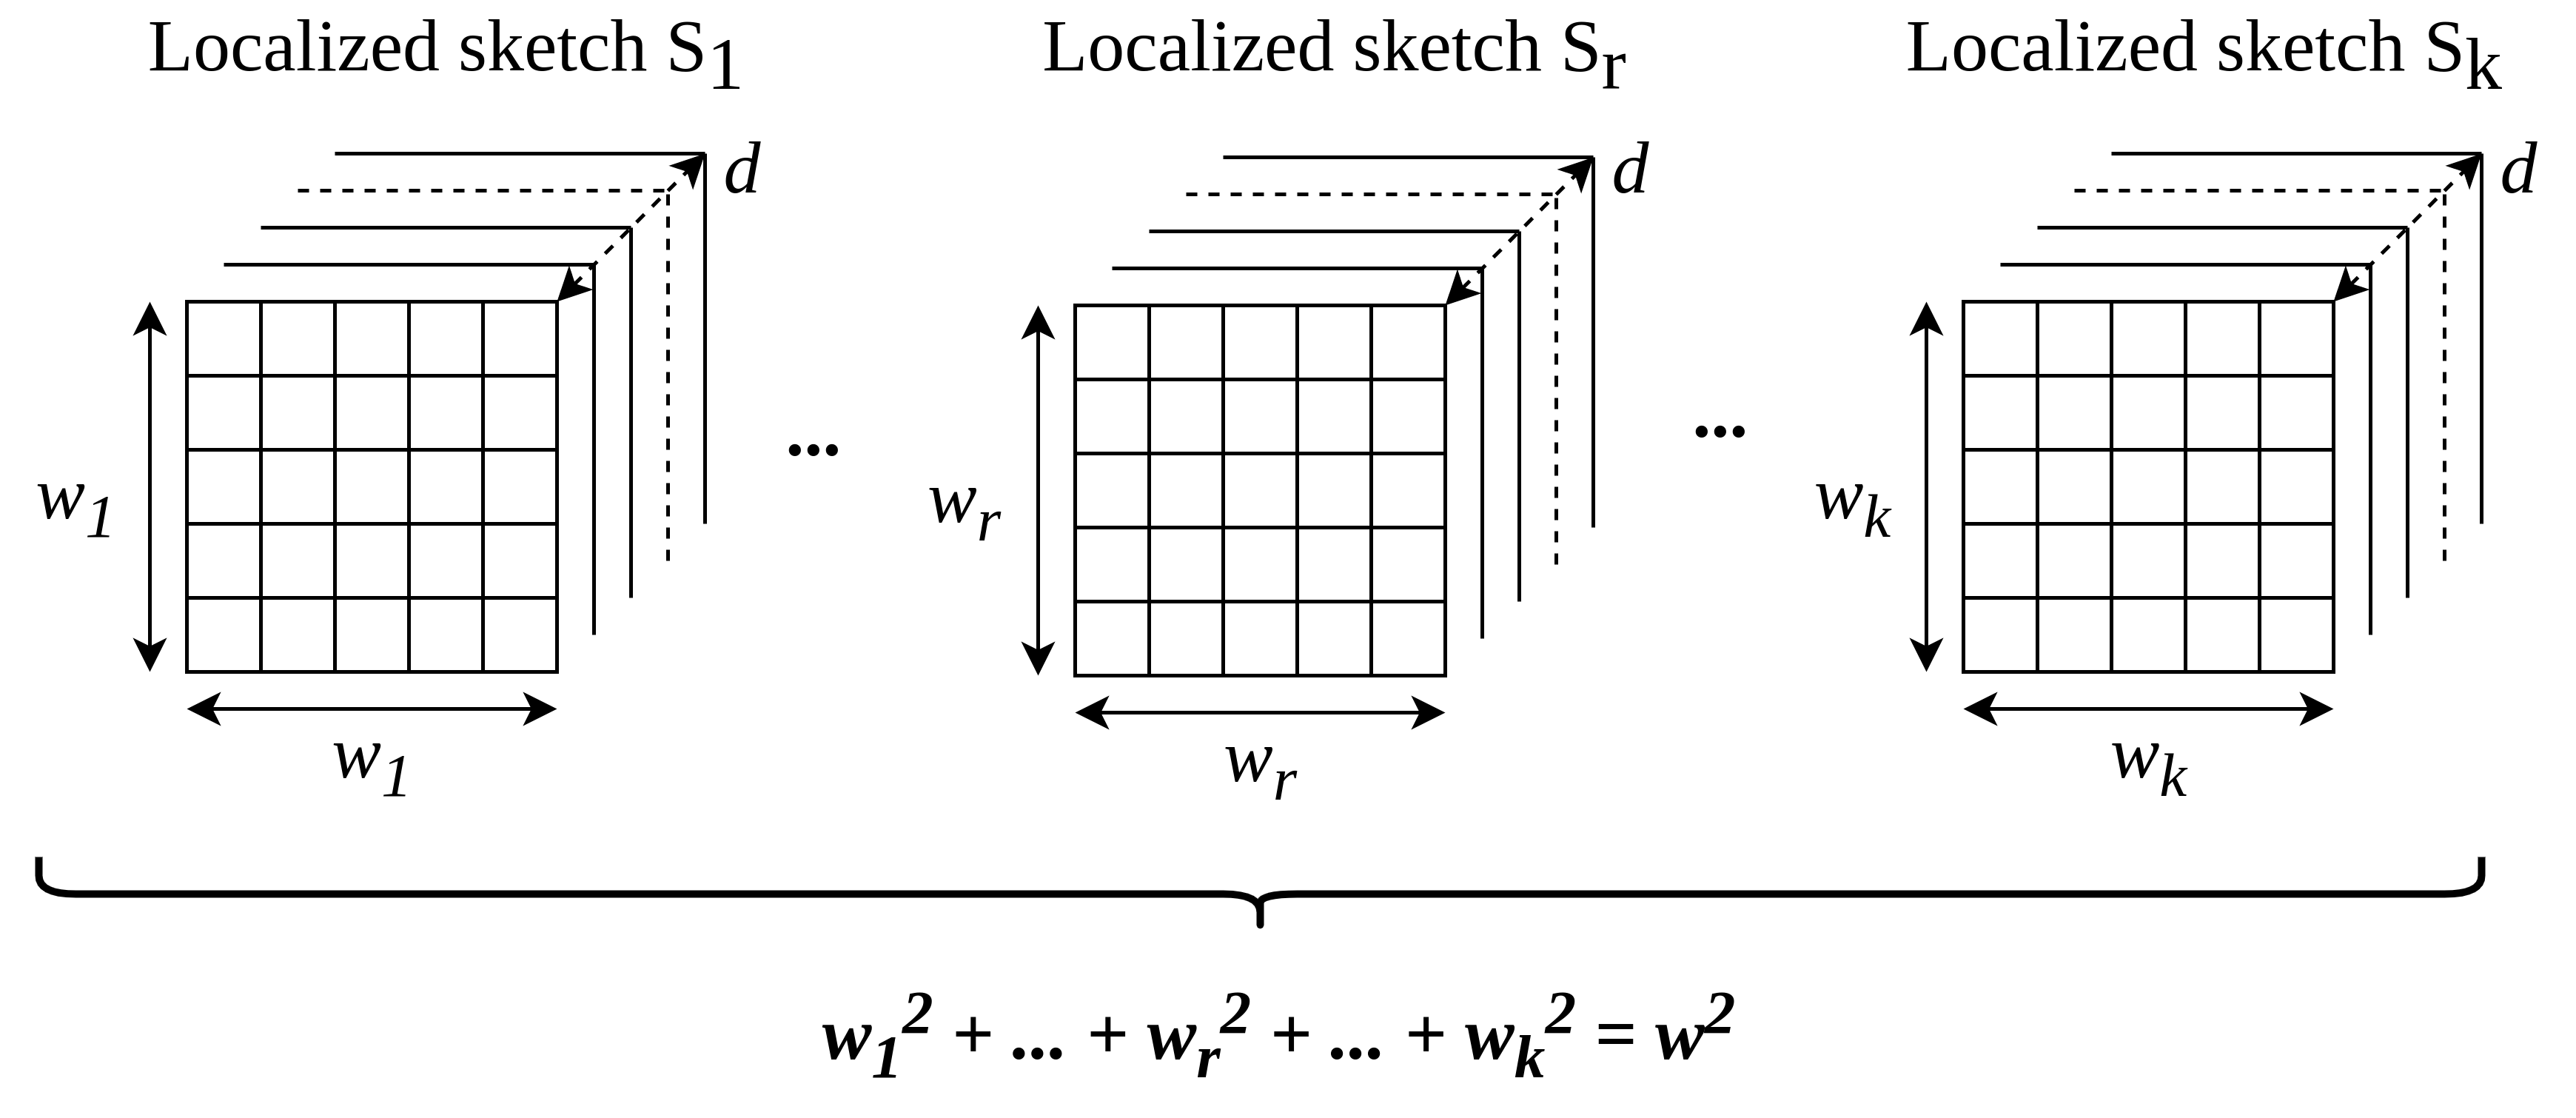
\includegraphics[width=0.5\textwidth]{img/kmatrix.png}}
    \caption{kMatrix sketch}
    \label{fig:kmatrix}
\end{figure}

\subsubsection*{Partitioning Algorithm}

Consider that the original sketch is partitioned into i sub-sketches. Let \(F(S_i)\) be the sum of the edge frequencies in the \(i\)th sketch and \(w_i\) be its width. If \((m,n)\) is an edge in the \(i\)th sketch, let \(f(m,n)\) and \(\bar{f}(m,n)\) be its frequency and expected frequency \eqref{eq:1} respectively. 

\begin{equation}
    \bar{f}(m,n) = \frac{F(S_i) - f(m,n)}{w_i}
    \label{eq:1}
\end{equation}

Then the expected relative error of the edge \((m,n)\) is given by \eqref{eq:2}.

\begin{equation}
    \bar{e}(m,n) = \frac{\bar{f}(m,n)}{f(m,n)} = \frac{F(S_i)}{f(m,n) . w_i} - \frac{1}{w_i}
    \label{eq:2}
\end{equation}

The overall relative error \(E_i\) of the sketch can be expressed as the sum of the expected relative errors of all the edges.

\begin{equation}
    E_i = \sum_{(m,n) \in S_i}^{} \bar{e}(m,n)
    \label{eq:3}
\end{equation}

Let the average frequency of a vertex \(m\) be \(\tilde{f}_v(m)\) and the estimated out-degree be \(\tilde{d}(m)\). Then the average frequency of the vertex would be \( \tilde{f}_v(m) / \tilde{d}(m) \). Therefore the total estimated frequencies of the partitioned sketch \(S_i\) can be expressed as \eqref{eq:4}.

\begin{equation}
    \tilde{F}(S_i) = \sum_{m \in S_i \: ; \: m \in V}^{} \tilde{f}_v(m)
    \label{eq:4}
\end{equation}

According to \eqref{eq:2}, \eqref{eq:3} and \eqref{eq:4}, the overall relative error of the sketch can be simplified to \eqref{eq:5}.

\begin{equation}
    E_i = \sum_{m \in S_i}^{} \frac{\tilde{d}(m) . \tilde{F}(S_i)}{w_i . (\tilde{f}_v(m) / \tilde{d}(m))} - \sum_{m \in S_i}^{} \frac{\tilde{d}(m)}{w_i}
    \label{eq:5}
\end{equation}

\(\tilde{d}(m)\) in the numerator accounts for the fact that \(O(\tilde{d}(m))\) edges are coming out of the vertex m.

When a sketch of width \(w\) is partitioned into two sketches of widths \(w_1\) and \(w_2\), the total error can be expressed as \(E = E_1 + E_2\). Let \(w_1 = w_2\). Then,

\begin{multline}
    E = \sum_{m \in S_1}^{} \frac{\tilde{d}(m) . \tilde{F}(S_i)}{w_1 . (\tilde{f}_v(m) / \tilde{d}(m))} + \sum_{m \in S_2}^{} \frac{\tilde{d}(m) . \tilde{F}(S_i)}{w_2 . (\tilde{f}_v(m) / \tilde{d}(m))}\\ - \sum_{m \in S_1 \cup S_2}^{} \frac{\tilde{d}(m)}{w_1}
    \label{eq:6}
\end{multline}

The \eqref{eq:6} can be further simplified as,

\begin{equation}
    E' = E . w_1 + \sum_{m \in S_1 \cup S_2}^{} \tilde{d}(m)
    \label{eq:7}
\end{equation}

where the value of \(E'\) is,

\begin{equation}
    E' = \sum_{m \in S_1}^{} \frac{\tilde{d}(m) . \tilde{F}(S_i)}{\tilde{f}_v(m) / \tilde{d}(m)} + \sum_{m \in S_2}^{} \frac{\tilde{d}(m) . \tilde{F}(S_i)}{\tilde{f}_v(m) / \tilde{d}(m)}
    \label{eq:8}
\end{equation}

Thus it can be shown that the overall error in \eqref{eq:7} can be minimized by choosing the smallest \(E'\) according to \eqref{eq:8}. Therefore the underlying idea behind the partitioning algorithm is to choose a data sample of the original stream and then repeatedly partition the available space between the vertices in the sample according to \eqref{eq:8}. After this partitioning phase, the streaming can begin and the edges that represented the vertices in the sample are put into their respective partitioned sketches.

A separate data structure has to be used in order to track the vertices belonging to different localized partition. However the extra cost of storing this information is negligible when compared with the advantages obtained with the sketch partitioning.